\chapter{Testing and Results}

In order to examine the performance and robustness of my approach, a serious of experiments target both individual functions and the integrated system has been conducted. The success rate and execution times are the two evaluation criteria.

In all experiments, I utilize the same platform as shown in Figure \ref{5.1}. It consists of a YuMi robot and an external camera (ZED Mini or ASUS Xtion). In order to maximize the accuracy, ZED Mini camera with highest resolution settings ($2208 \times 1242$) is chosen for all the experiments in this chapter. The marked shoe will be placed on the workbench within the area YuMi can reach. All tests were conducted under normal lighting conditions. 

\section{Shoe Detection and Pose Estimation}
The purpose of this part experiment is to assess the robustness of object detection and if the system can correctly compute adjustment locations or the centroid of the shoe hole.

The marked shoe will be placed at random location on the workbench for 10 times, together with other disturbing objects. For each location, I rotate the shoe 5 times to adjust its orientation. YOLO algorithm will be used to perform shoe detection and return the prediction probability and the bounding box. Its performance is illustrated in Table \ref{yolotest}.

\begin{table}[H]
\centering
\resizebox{\columnwidth}{!}{
\begin{tabular}{||c||c|c|c|c|c|c||}
\hline
 & \begin{tabular}[c]{@{}c@{}}Average \\ execution time\end{tabular} & \begin{tabular}[c]{@{}c@{}}Success \\ rate\end{tabular} & \begin{tabular}[c]{@{}c@{}}Average\\ probability\end{tabular} & \begin{tabular}[c]{@{}c@{}}Minimum \\ probability\end{tabular} & \begin{tabular}[c]{@{}c@{}}Maximum \\ probability\end{tabular} & \begin{tabular}[c]{@{}l@{}}Standard \\ deviation\end{tabular} \\ \hline
 \hline
Shoe detection & 0.067s & 50/50 & 0.65 & 0.36 & 0.96 & 0.17 \\ \hline
\end{tabular}}
\caption{The testing results of YOLO shoe detection}
\label{yolotest}
\end{table}

As can be seen, the shoe detection system achieved 100\% success rate in these 50 tests with high detection speed. The relatively large fluctuation of detection probability is due to several low readings. These low probabilities are obtained when the shoe is placed on the edge of the image captured by the camera, such as Figure \ref{yolotestexample}. Overall, the performance of shoe detection is desirable. 

\begin{figure}[H]
\centering
\subfigure[Low confidence when the shoe is placed on the edge of the image]{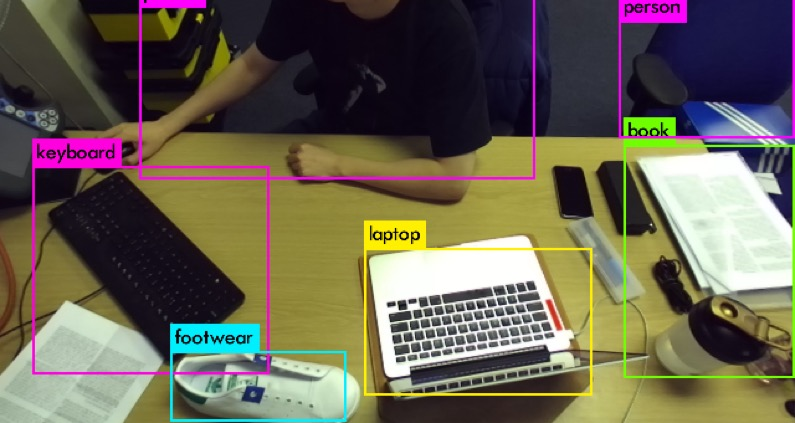
\includegraphics[width = 0.45\columnwidth]{TaR/yolot1.jpg}\label{yolotestexample}}
\subfigure[High confidence when the shoe is placed in the middle of the image]{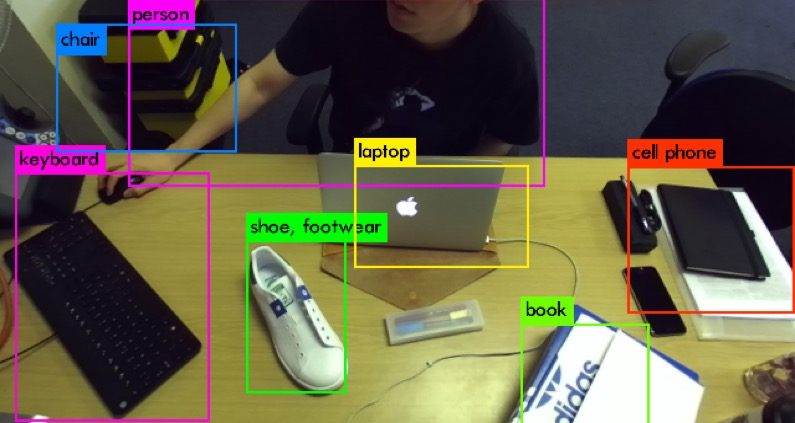
\includegraphics[width = 0.45\columnwidth]{TaR/yolot2.jpg}}
\caption{The examples of YOLO testing environments}
\end{figure}

Once YOLO detects a shoe, the following two situations will occur. When the shoe is vertically placed, the algorithm should publish the required four adjustment locations ($adr$, $adrr$, $adl$, and $adll$) to $TF$. If the shoe is in a good orientation, the 2D pixel coordinate of centroid of the shoe hole is supposed to be reported. Following tests will examine whether my approach can correctly classify the two situations and return the accurate results under the condition that YOLO can correctly detect the shoe.

\begin{table}[H]
\centering
\begin{tabular}{||c||c|c||}
\hline
 & Average execution time & Success rate \\ \hline \hline
Return adjustment locations & 0.01s & 20/20 \\ \hline
Return centroid coordinate & 0.046s & 30/30 \\ \hline
\end{tabular}
\caption{The testing results of situation classification}
\label{locationtest}
\end{table}

In the following experiment, I place the shoe vertically on the workbench for 20 times, and non-vertically for 30 times. Table \ref{locationtest} shows that my approach is able to classify the different situation with 100\% accuracy. Moreover, in most cases, the centorid location can be computed with high precision, as proved in Figure \ref{centroidresult}. 

\begin{figure}[H]
\centering
\subfigure[]{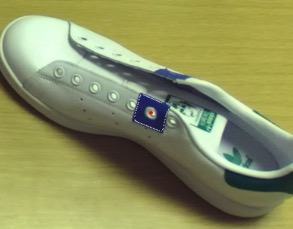
\includegraphics[height=3cm,keepaspectratio]{TaR/1.jpg}}
\subfigure[]{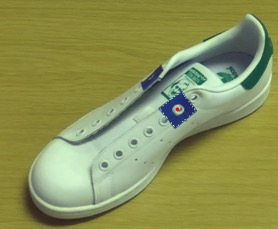
\includegraphics[height=3cm,keepaspectratio]{TaR/2.jpg}}
\subfigure[]{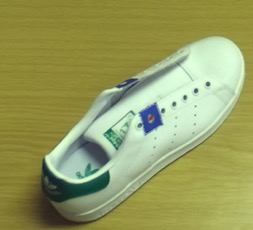
\includegraphics[height=3cm,keepaspectratio]{TaR/3.jpg}}
\subfigure[]{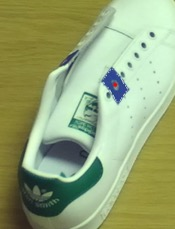
\includegraphics[height=3cm,keepaspectratio]{TaR/5.jpg}}
\subfigure[]{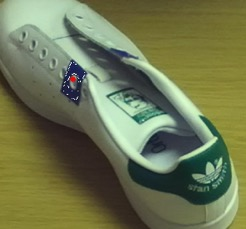
\includegraphics[height=3cm,keepaspectratio]{TaR/6.jpg}}
\subfigure[]{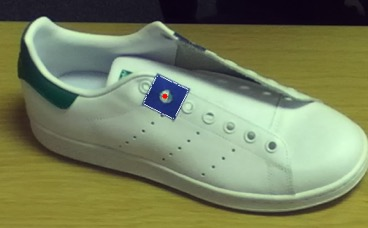
\includegraphics[height=3cm,keepaspectratio]{TaR/4.jpg}}
\caption{The examples of computed 2D pixel position of the shoe hole. The contour is drew in white, the centorid is marked in red.}
\label{centroidresult}
\end{figure}

Figure \ref{centroidresult} (e) is when the maximum error occurs. It can be discovered that there is a small offset between the red dot and the geometric center of shoe hole, which is considered to be acceptable.

\section{Shoe Pose Adjustment}
This section is to assess the performance of real shoe pose adjustment. Starting with four adjustment locations ($adr$, $adrr$, $adl$, and $adll$) being provided, YuMi will use both of its arms to adjust the orientation of the shoe. This feature was tested 15 times and the results are shown in Table \ref{adjusttest}.

\begin{table}[H]
\centering
\begin{tabular}{||c||c|c||}
\hline
 & Average execution time & Success rate \\ \hline \hline
Shoe pose adjustment & s & /15 \\ \hline
\end{tabular}
\caption{The testing results of situation classification}
\label{adjusttest}
\end{table}

any collisions?


\section{Insertion and Pulling of The Shoelace}
So far, the accuracy of YuMi's approaching pose for shoelace insertion still depends on two factors: the accuracy of estimation of shoe hole orientation, and the offset adjustment. Together with my motion planning algorithm, the real shoe insertion tests were carried out 15 times based on the condition that the 2D pixel centroid of the shoe hole and its contour area are correctly computed.

\begin{table}[H]
\centering
\begin{tabular}{||c||c|c||}
\hline
 & Average execution time & Success rate \\ \hline \hline
Shoelace insertion & s & /15 \\ \hline
Shoelace grabbing & s & /15 \\ \hline
\end{tabular}
\caption{The testing results of situation classification}
\label{insertnpull}
\end{table}

Table \ref{insertnpull}

\section{Integrated System Performance}

all of them 
